% report_31_01_2018.tex
% Omkar H. Ramachandran
% omkar.ramachandran@colorado.edu
%
% Documentation for hemispheric dependence in the Fermi Pass 8 data
%

\documentclass[english]{article}
\usepackage[T1]{fontenc}
\usepackage[latin9]{inputenc}
\usepackage{geometry}
\geometry{verbose,tmargin=1.5in,bmargin=1.5in,lmargin=1.5in,rmargin=1.5in}
\usepackage{babel}
\newcommand{\GeV}{\,{\rm GeV}}
\usepackage{graphicx}
\graphicspath{{./plots/}}

\begin{document}
\title{Hemispheric dependence of the pseudoscalar $Q$ in Pass 8 of the Fermi LAT data}
\author{Omkar H. Ramachandran}

\maketitle

\begin{abstract}
A recent study by Tashiro et al. (2015) proposed a mechanism through which the 
helicity of an extragalactc magnetic field could be estimated by measuring
a CP-odd pseudoscalar $Q$.
A significant observation in their study was the apparent dependence of
this pseudoscalar on the hemisphere where it is measured. 
In this study, we extend the original analysis using 100 weeks of data from 
Pass 8 of the Fermi Large Area Telescope (LAT) to better understand this 
dependence.
\end{abstract}

\section{Method and Setup}
\subsection{Setting up a Monte-Carlo simulation}
If there was no intervening magnetic field between source and detector, the
probability that a photon hits any point on the sphere is identical to the
corresponding probability at any other point.
Therefore, it is possible to model this by setting up a monte-carlo simulation
such that $\cos \theta$ and $\phi$ are uniformly distributed over $[-1,1]$ and
$[0,2\pi]$ respectively.
Figure \ref{fig:montecarlo} shows the measured value of $Q$ for a montecarlo
simulation with 10551 photons in the low energy bin, 1348 photons in the 
intermediate bin and 550 in the highest energy bin. This process was then
repeated 100 times and averaged.
\begin{figure}
	\label{fig:montecarlo}
	\centering
	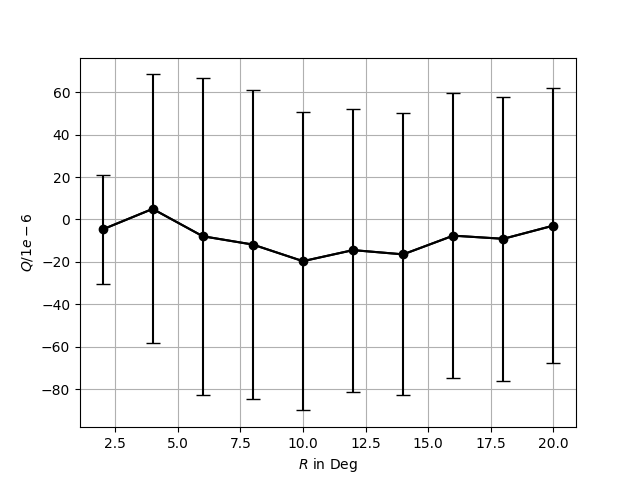
\includegraphics[scale=0.5]{montecarlo.png}
	\caption{Monte-Carlo simulation of the pseudoscalar $Q$ if there were no
	intervening field. It is evident from the plot that the mean value of $Q$
	always zero within the error-bars}
\end{figure}

\section{Calculating $Q$ from the Fermi Data}
\begin{figure}
	\label{fig:montecarlo}
	\centering
	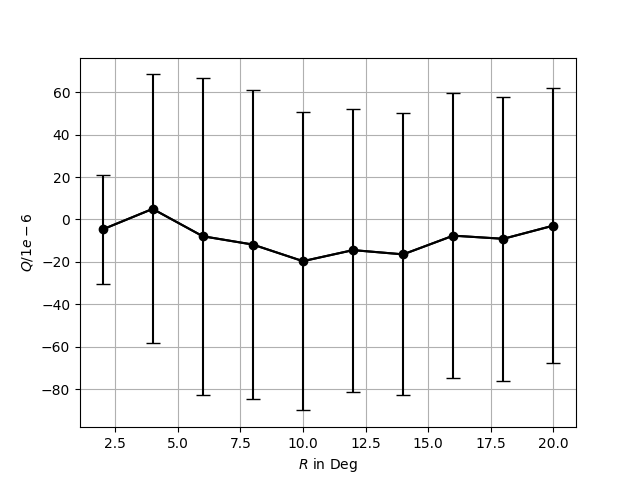
\includegraphics[scale=0.5]{montecarlo.png}
	\caption{Monte-Carlo simulation of the pseudoscalar $Q$ if there were no
	intervening field. It is evident from the plot that the mean value of $Q$
	always zero within the error-bars}
\end{figure}



\end{document}
